% % % % % % % % % % % % % % % % % % % % % % % % % % % % % % % % % % % % % % % % % % % %
%                                                                                     %
% Short Sectioned Assignment LaTeX Template Version 1.0 (5/5/12)                      %
% This template has been downloaded from: http://www.LaTeXTemplates.com               %
%                                                                                     %
% Original author:  Frits Wenneker (http://www.howtotex.com)                          %
%                                                                                     %
% Modified by: Fco Javier Sueza Rodríguez (fcosueza@disroot.org)                      %
%                                                                                     %
% Changes:                                                                            %
%	    - Custom Chapters, Sections and Subsections (titlesec package)                %
%           - Document type scrbook (oneside)                                         %
%           - Use babel-lang-spanish package and marvosym                             %
%           - Use hyperref, enumitem, tcolorbox and glossaries packages               %
%           - Use Time New Roman (mathptmx), Helvetic and Courier fonts               %
%                                                                                     %
% License: CC BY-NC-SA 3.0 (http://creativecommons.org/licenses/by-nc-sa/3.0/)        %
%                                                                                     %
% % % % % % % % % % % % % % % % % % % % % % % % % % % % % % % % % % % % % % % % % % % %

%-----------------------------------------------%
%	              Packages                  %
%-----------------------------------------------%

\documentclass[paper=a4, fontsize=11pt, oneside]{scrbook}

% ---- Text Input/Output ----- %

\usepackage[T1]{fontenc}
\usepackage[utf8]{inputenc}
\usepackage{mathptmx}
\usepackage[scaled=.92]{helvet}
\usepackage{courier}
\usepackage[indent=12pt]{parskip}

\usepackage{geometry}
\geometry{verbose,tmargin=3cm,bmargin=3cm,lmargin=2.6cm,rmargin=2.6cm}

% ---- Language ----- %

\usepackage[spanish]{babel}
\usepackage{marvosym}

% ---- Another packages ---- %

\usepackage{amsmath,amsfonts,amsthm}
\usepackage{graphics,graphicx}
\usepackage{titlesec}
\usepackage{fancyhdr}
\usepackage{tcolorbox}
\usepackage{hyperref}
\usepackage{enumitem}
\usepackage[automake]{glossaries}

%--------------------------------------------------------------------%
%                      Customizing Document                          %
%--------------------------------------------------------------------%


% ----------- Custom Chapters, Sections and Subsections -------------- %

\titleformat{\chapter}[display]
			{\bfseries\Huge}
			{Tema \ \thechapter} {0.5ex}
			{\vspace{1ex}\centering}

\titleformat{\section}[hang]
			{\bfseries\Large}
			{\thesection}{0.5em}{}

\titleformat{\subsection}[hang]
			{\bfseries\large}
			{\thesubsection}{0.5em}{}

\titleformat{\subsubsection}[hang]
			{\bfseries\large}
			{\thesubsubsection}{0.5em}{}

\hypersetup{
    colorlinks=true,
    linkcolor=black,
    urlcolor=magenta
}

% ------------------- Custom heaaders and footers ------------------- %

\pagestyle{fancyplain}

\fancyhead[]{}
\fancyfoot[L]{}
\fancyfoot[C]{}
\fancyfoot[R]{\thepage}

\renewcommand{\headrulewidth}{0pt} % Remove header underlines
\renewcommand{\footrulewidth}{0pt} % Remove footer underlines

\setlength{\headheight}{13.6pt} % Customize the height of the header

% --------- Numbering equations, figures and tables ----------------- %

\numberwithin{equation}{section} % Number equations within sections
\numberwithin{figure}{section} % Number figures within sections
\numberwithin{table}{section} % Number tables within sections

% ------------------------ New Commands ----------------------------- %

\newcommand{\horrule}[1]{\rule{\linewidth}{#1}} % Create horizontal rule command


%----------------------------------------------------------------------------------------
%	TÍTULO Y DATOS DEL ALUMNO
%----------------------------------------------------------------------------------------

\title{
\vspace{10ex}
\normalfont \normalsize
\huge \textbf{Tarea 5: Clasificación Jurídica de la Empresa y Trámites de Constitución}
}
\author{Francisco Javier Sueza Rodríguez}
\date{\normalsize\today}

%----------------------------------------------------------------------------------------
%                                     DOCUMENTO
%----------------------------------------------------------------------------------------
\begin{document}

\maketitle

\thispagestyle{empty}

\vspace{65ex}

\begin{center}
    \begin{tabular}{l l}
        \textbf{Centro}: & IES Aguadulce \\
        \textbf{Ciclo Formativo}: & Desarrollo Aplicaciones Web (Distancia)\\
        \textbf{Asignatura}: & Empresa e Iniciativa Emprendedora\\
        \textbf{Tema}: & Tema 5 - Clasificación Jurídica de la Empresa y Trámites de Constitució\\
    \end{tabular}
\end{center}

\newpage

\tableofcontents

\newpage

\section{Caso Práctico}
\textbf{Contigo S.L} es la empresa que han creado los chicos del supuesto práctico de esta unidad, se trata, como su nombre indica, de una Sociedad Limitada, porque reúnen los requisitos que la ley exige para su constitución, tiene una tramitación telemática y algunas ventajas fiscales. Han descartado otras formas jurídicas por las características de su empresa y sus circunstancias. Les hemos acompañado a lo largo de la unidad en los trámites de constitución y puesta en marcha de su negocio.

¡En esta tarea te toca a ti hacer lo mismo! Antes haremos algunos supuestos para repasar las formas jurídicas.

\section{Ejercicios}


\subsection{Ejercicio 1}
De los supuestos que se presentan a continuación, determina la forma jurídica más adecuada, justificando tu respuesta en no más de tres líneas:

\begin{enumerate}[label=\alph*)]
    \item Antonio, trabaja por cuenta ajena como desarrollador de aplicaciones multiplataforma. Ha creado una aplicación para la gestión de PYMES y siente que tiene los conocimientos y la experiencia laboral suficientes para montar su propio negocio en solitario. Quiere trabajar desde su domicilio para atender las necesidades de su familia y reducir gastos. Considera este proyecto una oportunidad y está muy ilusionado. Los riesgos son bajos porque es poca la inversión. La tramitación es la más sencilla de todas las formas jurídicas.

    \item El alumnado de un ciclo de informática ha trabajado en el módulo de EIE un proyecto empresarial para la instalación y mantenimiento de pantallas de visualización en centros públicos. Cuatro de ellos han decidido hacerlo realidad constituyendo una empresa de economía social. Todos son jóvenes (menores de 30 años), trabajarán en la empresa y aportarán el mismo capital, 1.000 euros cada uno. Prefieren no responder de las deudas de la actividad con su patrimonio y limitar su responsabilidad al capital aportado.

    \item Una sociedad limitada consolidada en el sector de las telecomunicaciones y valorada en 850.000 euros, desea mejorar su prestigio, internacionalizarse y absorber otras empresas de la competencia. Decide hacer una importante ampliación de capital y cambiar su forma jurídica a otra que responda a estas nuevas circunstancias.

    \item Susana y Marcos quieren dedicarse al asesoramiento informático integral para empresas y particulares. Se instalarán en un vivero local y como los primeros años prevén pocos beneficios y muchos gastos, han descartado la idea de constituirse como sociedad mercantil. Están dispuestos a tener una responsabilidad personal e ilimitada por las deudas de la sociedad, pero quieren que quede clara la aportación de cada uno y su participación en los beneficios. ¿Qué forma jurídica les recomendamos inicialmente? ¿Y cuándo los beneficios superen los 70.000 euros anuales y decidan separar su patrimonio personal de la marcha de la empresa?.
\end{enumerate}

\subsubsection{Solución}


A continuación se indican las formas jurídicas más adecuadas para los casos enumerados en el enunciado:

\begin{enumerate}[label=\alph*)]
    \item La forma más idónea para la empresa de Antonio es la de \textbf{empresa individual} o \textbf{autónomo}, ya que va a ejercer el solo el desarrollo de la actividad comercial, no requiere capital mínimo y además es la más sencilla de tramitar.

    \item En este caso, la mejor forma jurídica sería la de una \textbf{Sociedad Limitada Laboral}, ya que estamos hablando de 4 socios, que además van a ser trabajadores de la empresa y que no quieren responder con su patrimonio, limitando la responsabilidad al capital aportado.

    \item Dadas las nuevas circunstancias de la empresa y los objetivos que tiene forma jurídica más idónea sería la de
    una \textbf{Sociedad Anónima}, ya que esto permitiría recabar más inversiones, además, con la absorción de nuevas empresas, la trasmisión de forma fácil de acciones sería una elemento a tener en cuenta.

    \item La forma jurídica más idónea para esta situación sería una \textbf{Sociedad Civil}, ya que no requiere ningún tipo de inversión inicial, que no habría que sumar a los gatos previstos y además cada socio participa de los beneficios según su aportación, uno de los requisitos de Susana y Marcos. Una vez que la empresa tenga beneficios de más de 70.000 € al año, podrían constituirse como \textbf{Sociedad Limitada}, por lo que la responsabilidad por las deudas contraídas con la empresa no afectaría a su patrimonio personal.
\end{enumerate}

\subsection{Ejercicio 2}
Vamos a completar en esta tarea un nuevo apartado del plan de negocio que estás elaborando, se llama: LA FORMA JURÍDICA.

Te proponemos que contestes a esta actividad con la siguiente plantilla, aunque puedes elegir otro formato:

\begin{itemize}
    \item  La denominación social, el nombre comercial de la empresa y su logo.
    \item El domicilio social y la ciudad en la que se ubicará la empresa.
    \item Las personas emprendedoras: Las personas que la integran en calidad de socios y su aportación (capital, trabajo, bienes…), determinando el tipo de responsabilidad (personal, ilimitada, limitada...).
    \item Puedes concretar también qué otras personas van a componer el equipo y si se trata de colaboradores, trabajadores, asesores, gestores...
\end{itemize}

\subsubsection{Solución}

Mi empresa se llama \textbf{Site Wise}, una empresa dedicada al desarrollo de aplicaciones web y al asesoramiento para la adopción de TIC por parte de PyMES. El logotipo es el que podemos ver en la siguiente imagen.

 \begin{figure}[H]
    \centering
    
\includegraphics[scale=0.33]{logo-empresa.png}
\end{figure}

La empresa tiene su domicilio fiscal en \textbf{Avd. de Dilar n10}, ubicado en la localidad de \textbf{Granada}, provincia de \textbf{Granada}.

La \textbf{forma jurídica} elegida ha sido la de \textbf{Sociedad Limitada}. Esta elección se ha llevado a cabo ya que es un empresa pequeña, que no tiene una capital de inversión inicial elevado, dado su actividad. Por este motivo, aunque ya solo requiera 1€ como capital inicial, se podría disponer de los 3000€ iniciales para así no tener que destinar un 20\% de los beneficios iniciales. Además, siendo yo en único socio, tampoco estaría interesado en responder con mi patrimonio en caso de que se contrajeran deudas.

La empresa está integrada por \textbf{un socio trabajador}, que soy yo, además de \textbf{5 trabajadores}, necesarios para el correcto desarrollo de actividad de la empresa. Los trabajadores de componen de \textbf{2 desarrolladores}, \textbf{1 diseñador gráfico}, \textbf{1 administrador de sistema} y \textbf{1 product manager}. Así mismo yo desarrollare la labor de \textbf{desarrollador}.

El \textbf{capital social inicial} de la empresa se estima en \textbf{10000€}, incluyendo los materiales que deben comprarse para el desarrollo de la actividad y los 3000€ iniciales para evitar dedicar el 20\% de los beneficios a obtener esa cantidad.

Al haber elegido como forma jurídica la de \textbf{Sociedad Limitada}, la responsabilidad antes las deudas sociales es de \textbf{los socios}, en esta caso mía ya que soy el único socio, aunque esta responsabilidad se limitará al capital aportado.

\subsection{Ejercicio 3}
En este apartado haremos lo mismo que hicieron los protagonistas del supuesto práctico del tema (te invitamos a que lo repases en la unidad): 	Rellena unas fichas con los trámites de constitución de la empresa de la que estás elaborando el plan de negocio.


\subsubsection{Solución}
Los\textbf{ tramites de constitución} que se han tenido que realizar son:
\begin{figure}[H]
    \centering
    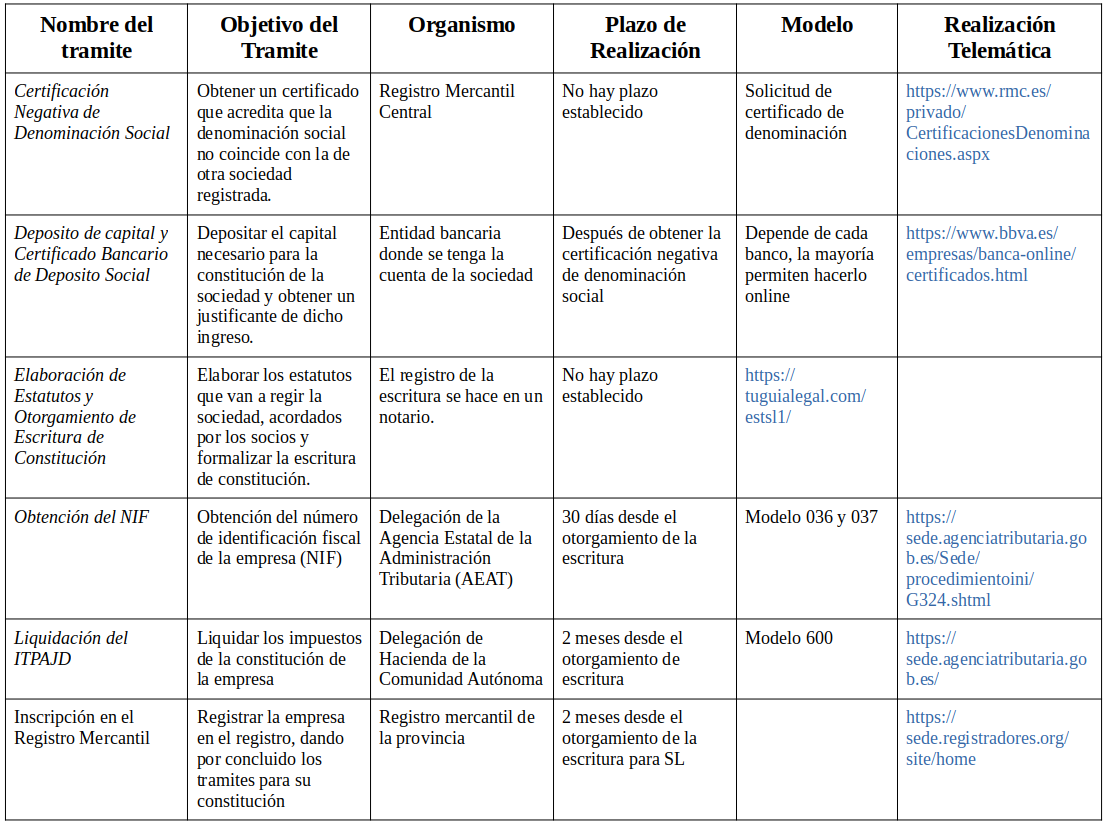
\includegraphics[scale=0.48]{tramites-constitucion.png}
\end{figure}

Una vez \textbf{constituida la empresa}, debemos realizar un conjunto de trámites para la puesta en marcha de la empresa. Estos trámites, conocidos como \textbf{trámites de puesta en marcha}, se realizan en diferentes administraciones.

A continuación, se detallan los trámites que se han tenido que realizar organizados por administración.

\subsubsection*{Delegación de la Agencia Estatal de la Administración Tributaria}
\begin{itemize}
    \item \textbf{Dirección}: Avenida de la Constitución, 1. 18071, Granada, Granada
    \item \textbf{Web}: \url{https://sede.agenciatributaria.gob.es/}
    \item \textbf{Teléfono}: 958 29 44 11
\end{itemize}

\begin{figure}[H]
    \centering
    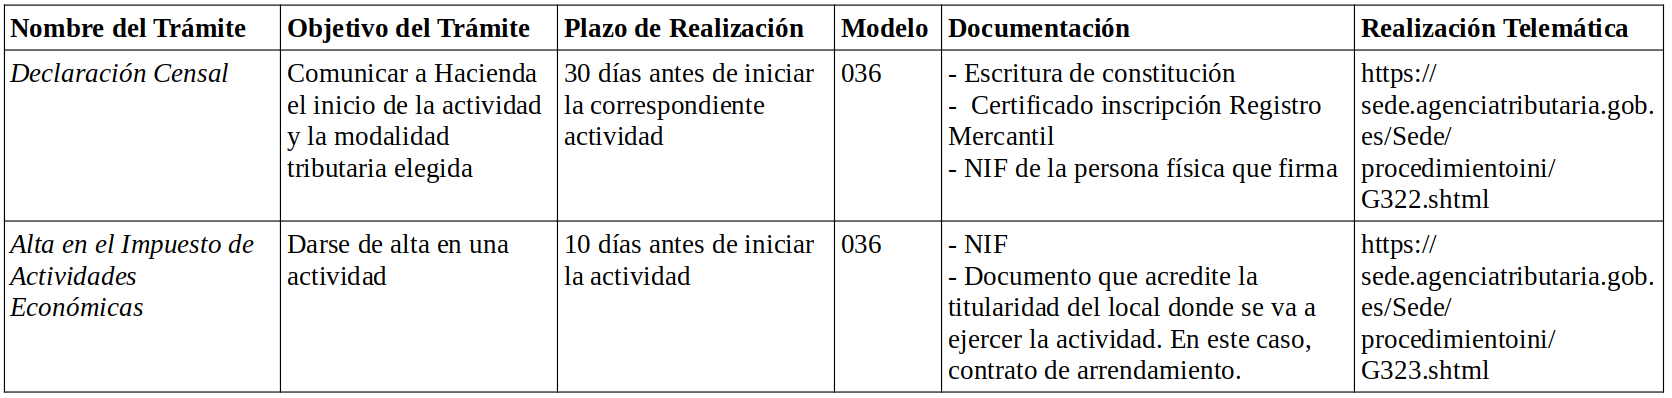
\includegraphics[scale=0.36]{tramites-AIE.png}
\end{figure}

\subsubsection*{Tesorería General de la Seguridad Social}
\begin{itemize}
    \item \textbf{Dirección}: Calle Gran Vía de Colón 23 18001 Granada (Granada)
    \item \textbf{Web}: \url{https://www.seg-social.es/wps/portal/wss/internet/Inicio}
    \item \textbf{Teléfono}: 901 50 20 50
\end{itemize}

\begin{figure}[H]
    \centering
    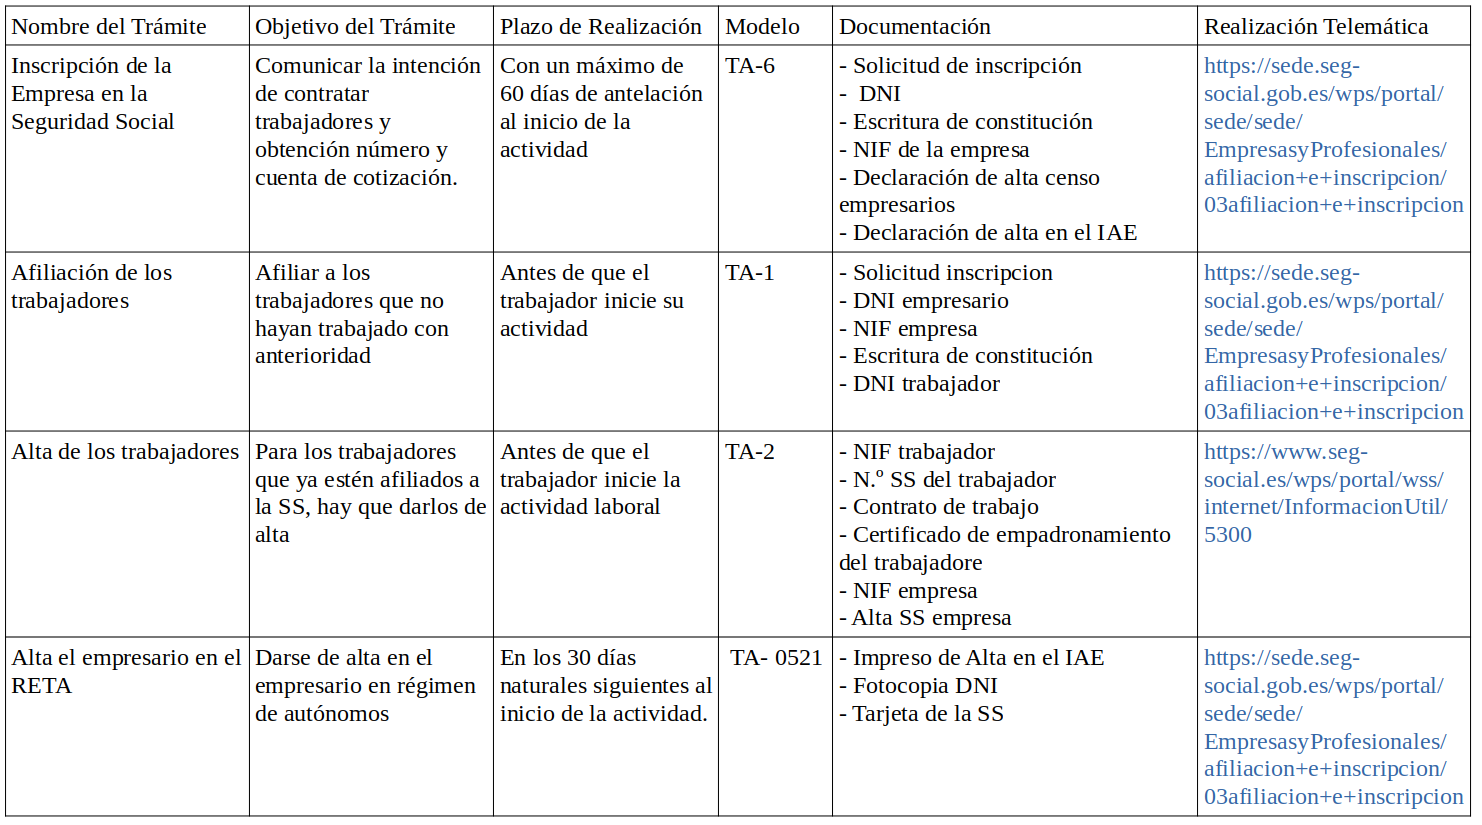
\includegraphics[scale=0.40]{tramites-SS.png}
\end{figure}

\subsubsection*{Trámites Laborales}

\begin{itemize}
    \item \textbf{En la Administración Laboral}
    \begin{itemize}
        \item \textbf{Nombre}: Delegación Territorial de Empleo, Empresa y Trabajo Autónomo en Granada
        \item \textbf{Dirección}: Calle Joaquina Eguaras 2 18013 Granada (Granada)
        \item \textbf{Web}: \url{https://www.mites.gob.es/}
        \item \textbf{Teléfono}: 958 02 73 23

        \begin{figure}[H]
            \centering
            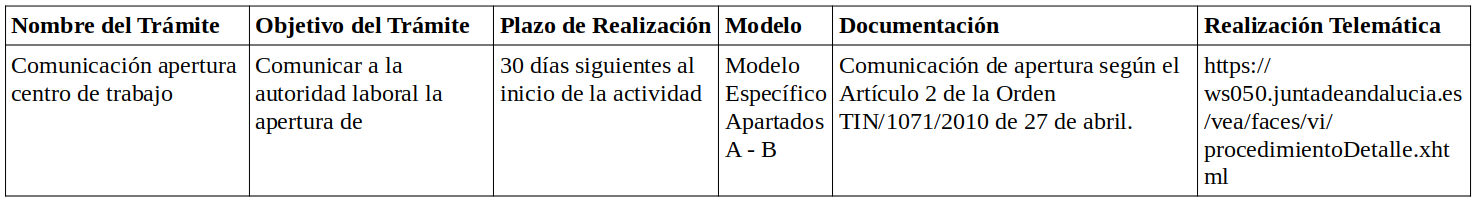
\includegraphics[scale=0.38]{tramites-laboral.png}
        \end{figure}
    \end{itemize}
    \item \textbf{En el SEPE}:
    \begin{itemize}
        \item \textbf{Dirección}:  C. Sos del Rey Católico, 3, Genil, 18006 Granada
        \item \textbf{Web}: \url{https://www.sepe.es/}
        \item \textbf{Teléfono}: 958 90 05 98

        \begin{figure}[H]
            \centering
            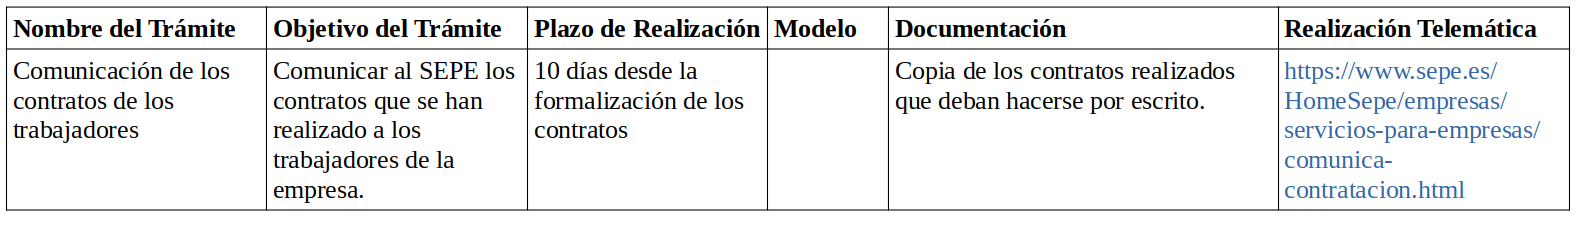
\includegraphics[scale=0.36]{tramites-SEPE.png}
        \end{figure}
    \end{itemize}

\end{itemize}
% Bibliography

%\newpage
%\bibliography{citas}
%\bibliographystyle{unsrt}

\end{document}